\subsection{Stimulus geometry}\label{sec:geometry}

\begin{table}[t]
\centering\footnotesize
\caption{Geometry of the ten stimulus sets, from the image files. Relative variances of coordinates $2, \dots, d$ (the first is 1); PR, participation ratio of the $d$ variances; NN, median nearest-neighbour distance over the median pairwise distance; last, standard deviation of the smallest coordinate over the median nearest-neighbour distance.}\label{tab:geometry}
\begin{tabular}{llp{6.6cm}ccc}
\toprule
set & mouse, date & relative variances & PR & NN & last \\
\midrule
8D & MP030 06-07 & 0.912, 0.733, 0.627, 0.496, 0.340, 0.328, 0.251 & 6.7 & 0.260 & 0.64 \\
8D & MP031 07-02 & 0.793, 0.675, 0.545, 0.345, 0.286, 0.253, 0.047 & 5.9 & 0.238 & 0.33 \\
8D & MP032 08-10 & 0.572, 0.549, 0.350, 0.261, 0.180, 0.012, 0.002 & 4.6 & 0.180 & 0.11 \\
8D & MP032 09-15 & 0.793, 0.717, 0.573, 0.443, 0.310, 0.266, 0.107 & 6.2 & 0.245 & 0.47 \\
8D & MP033 08-22 & 0.835, 0.497, 0.412, 0.089, 0.019, 0.008, 0.005 & 3.9 & 0.136 & 0.23 \\
8D & MP034 09-15 & 0.807, 0.726, 0.674, 0.549, 0.440, 0.319, 0.223 & 6.8 & 0.266 & 0.58 \\
4D & MP032 09-22 & 0.711, 0.612, 0.315 & 3.5 & 0.071 & 3.46 \\
4D & MP033 09-19 & 0.925, 0.570, 0.111 & 3.1 & 0.059 & 2.50 \\
4D & MP033 09-22 & 0.699, 0.608, 0.391 & 3.6 & 0.071 & 3.83 \\
4D & MP034 09-20 & 0.881, 0.568, 0.284 & 3.4 & 0.063 & 3.61 \\
\bottomrule

\end{tabular}
\end{table}

The four 4D sets are alike (Table~\ref{tab:geometry}), with participation ratios \PRFourMin{} to \PRFourMax{}. The six 8D sets are not: their participation ratios range from \PREightMin{} to \PREightMax{}, and in two of them (MP032 2017-08-10, MP033 2017-08-22) the last two or three coordinates carry less than 2\% of the variance of the first. In every 8D set the smallest coordinate has a standard deviation of only \SDNNEightMin{} to \SDNNEightMax{} times the median nearest-neighbour distance, itself \NNEightMin{} to \NNEightMax{} of the median pairwise distance: 2,800 stimuli do not sample short distances in eight dimensions, and smoothness is a short-distance property. At the scales these stimuli resolve, the sets are also lower-dimensional than nominal: the nearest-neighbour dimension is \DnnFourMin{} to \DnnFourMax{} in the 4D sets and \DnnEightMin{} to \DnnEightMax{} in the 8D sets (\DnnWhiteFourMin{} to \DnnWhiteFourMax{} and \DnnWhiteEightMin{} to \DnnWhiteEightMax{} in whitened coordinates), against \DnnGaussFourMin{} to \DnnGaussFourMax{} and \DnnGaussEightMin{} to \DnnGaussEightMax{} for Gaussian points with the same coordinate variances and the same numbers of points (\DnnGaussIsoFourMin{} to \DnnGaussIsoFourMax{} and \DnnGaussIsoEightMin{} to \DnnGaussIsoEightMax{} for isotropic ones, the control for whitened coordinates).

\subsection{Window exponents of Mat\'ern codes}

\begin{figure}[t]
\centering
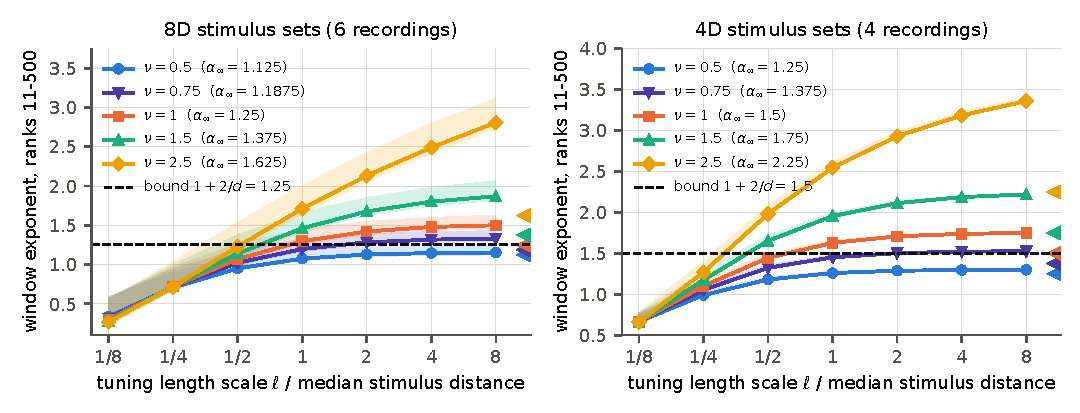
\includegraphics[width=0.94\textwidth]{figures/fig1.pdf}
\caption{Ranks 11--500 window exponent of noise-free Mat\'ern codes (infinitely many neurons) on the real stimulus coordinates, against the tuning length scale. Lines: median over the stimulus sets; bands: range over the sets. Arrowheads on the right: $\alpha_\infty = 1 + 2\nu/d$. Dashed line: the bound $1 + 2/d$. Deterministic. Table~\ref{tab:sens} gives the effect of finite populations, the rank window, the metric and the number of stimuli.}\label{fig:window}
\end{figure}

\begin{table}[t]
\centering\footnotesize
\caption{Ranks 11--500 window exponent of noise-free Mat\'ern codes (infinitely many neurons) on the real stimulus coordinates: range over the six 8D and the four 4D stimulus sets. Deterministic; no sampling error.}\label{tab:window}
\setlength{\tabcolsep}{3.5pt}
\begin{tabular}{ccc*{7}{c}}
\toprule
& & & \multicolumn{7}{c}{length scale $\ell$ / median pairwise distance} \\
\cmidrule(lr){4-10}
$d$ & $\nu$ & $\alpha_\infty$ & 1/8 & 1/4 & 1/2 & 1 & 2 & 4 & 8 \\
\midrule
8 & 0.5 & 1.125 & 0.30--0.59 & 0.67--0.90 & 0.93--1.09 & 1.05--1.18 & 1.10--1.22 & 1.12--1.23 & 1.12--1.24 \\
8 & 0.75 & 1.1875 & 0.27--0.58 & 0.68--0.94 & 0.99--1.19 & 1.17--1.33 & 1.25--1.39 & 1.28--1.42 & 1.29--1.43 \\
8 & 1 & 1.25 & 0.26--0.57 & 0.68--0.97 & 1.04--1.26 & 1.26--1.45 & 1.38--1.55 & 1.44--1.60 & 1.46--1.63 \\
8 & 1.5 & 1.375 & 0.23--0.56 & 0.67--1.00 & 1.10--1.38 & 1.41--1.67 & 1.62--1.85 & 1.75--1.98 & 1.82--2.07 \\
8 & 2.5 & 1.625 & 0.21--0.55 & 0.67--1.04 & 1.18--1.54 & 1.64--2.01 & 2.05--2.42 & 2.41--2.80 & 2.73--3.11 \\
\addlinespace
4 & 0.5 & 1.25 & 0.64--0.76 & 0.97--1.04 & 1.17--1.21 & 1.25--1.28 & 1.28--1.30 & 1.29--1.31 & 1.30--1.31 \\
4 & 0.75 & 1.375 & 0.63--0.77 & 1.03--1.12 & 1.31--1.36 & 1.45--1.48 & 1.50--1.52 & 1.52--1.53 & 1.52--1.54 \\
4 & 1 & 1.5 & 0.62--0.77 & 1.08--1.18 & 1.43--1.49 & 1.62--1.66 & 1.70--1.73 & 1.73--1.75 & 1.75--1.76 \\
4 & 1.5 & 1.75 & 0.62--0.77 & 1.14--1.28 & 1.63--1.72 & 1.95--2.00 & 2.11--2.14 & 2.18--2.21 & 2.21--2.23 \\
4 & 2.5 & 2.25 & 0.61--0.78 & 1.23--1.40 & 1.96--2.09 & 2.53--2.62 & 2.91--2.98 & 3.17--3.23 & 3.34--3.40 \\
\bottomrule

\end{tabular}
\end{table}

With infinitely many neurons the border codes ($\nu = 1$) give window exponents from \WinBorderEightMin{} to \WinBorderEightMax{} at $d = 8$ (bound 1.25) and from \WinBorderFourMin{} to \WinBorderFourMax{} at $d = 4$ (bound 1.50) (Figure~\ref{fig:window}, Table~\ref{tab:window}). They lie below the bound in every stimulus set for $\ell \le \CrossBelowEight$ at $d = 8$ and $\ell \le \CrossBelowFour$ at $d = 4$, and above it in every set for $\ell \ge \CrossAboveEight$ at $d = 8$ and $\ell \ge \CrossAboveFour$ at $d = 4$. The smoothness of these codes is fixed; the length scale moves the exponent across the bound, as Example~3 of \cite{stringer2019} anticipates for a single tuning radius. The stimulus set matters as well: at $\ell = 1$ the border code gives \WinBorderEightLOneMin{} to \WinBorderEightLOneMax{} across the 8D sets, the larger values in the sets with the smaller participation ratios, and \WinBorderFourLOneMin{} to \WinBorderFourLOneMax{} across the 4D sets. Differentiable codes fall below the bound at short length scales: at $\ell = 1/4$ the largest exponent over the 8D sets is \WinSmoothEightLQuarterMax{} for $\nu = 1.5$ and \WinSmootherEightLQuarterMax{} for $\nu = 2.5$, and over the 4D sets \WinSmoothFourLQuarterMax{} and \WinSmootherFourLQuarterMax{}. At long length scales they overshoot their own asymptotic exponent ($\nu = 2.5$ at $d = 4$ reaches \WinSmootherFourMax{} against $\alpha_\infty = 2.25$). Codes of fixed smoothness also reproduce the ordinal pattern that Stringer et al.\ predicted: in all \OrdinalTotal{} combinations of $\nu$ and $\ell$, every 4D set gives a larger exponent than every 8D set.

\subsection{How far these statements carry}

\begin{table}[t]
\centering\footnotesize
\caption{Ranks 11--500 window exponent of the border codes ($\nu = 1$) and of codes below the border ($\nu = 0.75$) under changes of the computation: range over the stimulus sets, with the number of sets above the bound $1 + 2/d$ in parentheses. $N = \infty$: Table~\ref{tab:window}. $N = 8{,}704$: mean over finite populations. 101--500: the same spectra fitted over ranks 101--500. Whitened: coordinates scaled to unit variance. $P$: mean over 4 random subsets of the stimuli.}\label{tab:sens}
\setlength{\tabcolsep}{3pt}
\begin{tabular}{ccc*{6}{c}}
\toprule
$d$ & $\nu$ & $\ell$ & $N = \infty$ & $N = 8{,}704$ & ranks 101--500 & whitened & $P = 1{,}400$ & $P = 2{,}000$ \\
\midrule
8 & 1 & 1 & 1.26--1.45 (6) & 1.24--1.44 (5) & 1.19--1.35 (2) & 1.13--1.19 (0) & 1.20--1.41 (2) & 1.24--1.43 (4) \\
8 & 1 & 4 & 1.44--1.60 (6) & 1.42--1.59 (6) & 1.30--1.43 (6) & 1.30--1.36 (6) & 1.38--1.56 (6) & 1.41--1.58 (6) \\
8 & 1 & 8 & 1.46--1.63 (6) & 1.44--1.62 (6) & 1.31--1.44 (6) & 1.33--1.38 (6) & 1.41--1.59 (6) & 1.44--1.61 (6) \\
8 & 0.75 & 4 & 1.28--1.42 (6) & 1.26--1.40 (6) & 1.13--1.24 (0) & 1.17--1.21 (0) & 1.21--1.36 (3) & 1.25--1.39 (6) \\
8 & 0.75 & 8 & 1.29--1.43 (6) & 1.27--1.41 (6) & 1.13--1.25 (0) & 1.18--1.23 (0) & 1.22--1.37 (4) & 1.26--1.40 (6) \\
\addlinespace
4 & 1 & 1 & 1.62--1.66 (4) & 1.62--1.66 (4) & 1.62--1.64 (4) & 1.60--1.63 (4) & 1.60--1.65 (4) & 1.61--1.65 (4) \\
4 & 1 & 4 & 1.73--1.75 (4) & 1.73--1.75 (4) & 1.66--1.67 (4) & 1.74--1.75 (4) & 1.72--1.74 (4) & 1.73--1.75 (4) \\
4 & 1 & 8 & 1.75--1.76 (4) & 1.74--1.76 (4) & 1.66--1.67 (4) & 1.76--1.76 (4) & 1.73--1.75 (4) & 1.74--1.76 (4) \\
4 & 0.75 & 4 & 1.52--1.53 (4) & 1.51--1.53 (4) & 1.43--1.44 (0) & 1.53--1.53 (4) & 1.48--1.50 (1) & 1.50--1.52 (4) \\
4 & 0.75 & 8 & 1.52--1.54 (4) & 1.51--1.53 (4) & 1.43--1.44 (0) & 1.53--1.54 (4) & 1.49--1.51 (1) & 1.51--1.52 (4) \\
\bottomrule

\end{tabular}
\end{table}

Table~\ref{tab:sens} tests these statements against the choices behind them. With 8,704 neurons the window exponents are mostly lower: over the \FinCells{} computed cells the mean shift ranges from \FinShiftMin{} to \FinShiftMax{}, and the \FinHigherN{} cells that rise are codes with $\nu = 1.5$ or $2.5$; between populations the standard deviation is only \FinSDMin{} to \FinSDMax{}. The border codes then lie below the bound in every set for $\ell \le \FinCrossBelowEight$ at $d = 8$ and $\ell \le \FinCrossBelowFour$ at $d = 4$, and above it in every set for $\ell \ge \FinCrossAboveEight$ at $d = 8$ and $\ell \ge \FinCrossAboveFour$ at $d = 4$ ($\ell = 1/8$ was not computed at finite $N$); at $\ell = 1$ they give \FinOneEightMin{} to \FinOneEightMax{} across the 8D sets, with \FinOneNearEight{} within 0.005 of the bound or below it. In the unwhitened coordinates they reach the reported exponents, 1.49 at $d = 8$ and 1.65 at $d = 4$, in \FinReachEight{} of the six 8D sets and in \FinReachAllFour{} four 4D sets, over the length scales computed (up to $\ell = 8$). The 8D count rests on a small margin: \FinReachMarginSetEight{} reaches \FinReachMarginEight{} above 1.49, with a standard deviation of \FinReachMarginSDEight{} over its \FinReachMarginREight{} populations. In whitened coordinates no 8D border code reaches 1.49: the largest value, with infinitely many neurons, is \WhiteBorderEightMaxAll{}, at $\ell = \WhiteBorderEightMaxAllEll$, the longest length scale computed. The 4D sets still reach 1.65 there (\WhiteBorderFourLEightMin{} to \WhiteBorderFourLEightMax{} at $\ell = 8$). For non-identification an existence statement in one metric suffices, but the 8D count holds only in the unwhitened metric.

For $\nu = 0.75$ the expected squared gradient diverges and $\alpha_\infty = 1 + 1.5/d$ lies below the bound (1.1875 at $d = 8$, 1.375 at $d = 4$). Over ranks 11--500, in the unwhitened coordinates and at 2,800 stimuli, these codes nevertheless exceed the bound at $\ell = 4$ in every set, with infinitely many neurons (\WinMidEightLFourMin{} to \WinMidEightLFourMax{} at $d = 8$, \WinMidFourLFourMin{} to \WinMidFourLFourMax{} at $d = 4$) and with 8,704 neurons in \FinMidAbovePhraseEight{} and \FinMidAbovePhraseFour{}. This is an existence statement for that window, that metric and that number of stimuli, and each matters. Over ranks 101--500 all \SubMidAboveCount{} cells of $\nu = 0.75$ that lie above the bound over ranks 11--500 fall below it (at $\ell = 4$: \SubMidEightLFourMin{} to \SubMidEightLFourMax{} at $d = 8$, \SubMidFourLFourMin{} to \SubMidFourLFourMax{} at $d = 4$). The spectra are curved: for $\ell \ge 1$ at $d = 8$ the ranks 11--100 exponent exceeds the ranks 101--500 exponent by a median of \CurvMedEight{} (over all cells the difference ranges from \CurvMin{} to \CurvMax{}), and for the \CurvBorderReachN{} border-code spectra that reach 1.49 in the 8D sets by \CurvBorderReachMin{} to \CurvBorderReachMax{}. We did not compute sub-window exponents of the recorded spectra, so whether spectra of this shape could stand in for the recorded ones is not tested here; the argument needs only that they give the same ranks 11--500 exponent. In whitened coordinates the $\nu = 0.75$ codes at $\ell = 4$ give \WhiteMidEightLFourMin{} to \WhiteMidEightLFourMax{} at $d = 8$, above the bound in \WhiteMidAboveEightWord{} of the six sets, while the 4D sets hardly change (\WhiteMidFourLFourMin{} to \WhiteMidFourLFourMax{}). The border codes keep landing on both sides in whitened coordinates: at $d = 8$ they give \WhiteBorderEightLOneMin{} to \WhiteBorderEightLOneMax{} at $\ell = 1$ and \WhiteBorderEightLEightMin{} to \WhiteBorderEightLEightMax{} at $\ell = 8$. With fewer stimuli the exponents fall: at $\ell = 4$ the 8D sets give \SubPOneThousandFourHundredMidEightLFourMin{} to \SubPOneThousandFourHundredMidEightLFourMax{} at $P = 1{,}400$ (above the bound in \SubPOneThousandFourHundredMidAboveEight{} of six sets) and \SubPTwoThousandMidEightLFourMin{} to \SubPTwoThousandMidEightLFourMax{} at $P = 2{,}000$ (above the bound in \SubPTwoThousandMidAboveEight{}; in \SubPTwoThousandMarginSet{} by only \SubPTwoThousandMarginMin{}, with a standard deviation over subsets of \SubPTwoThousandMarginSD{} and one subset at \SubPTwoThousandMarginSubMin{}). The subsets sample the same operator, so at 2,800 stimuli the window exponent still depends on the number of stimuli; its limit as $P$ grows, the window exponent of the operator eigenvalues at ranks 11--500, cannot be computed from these stimulus sets. Solving $w = 1 + 2\nu/d_{\mathrm{eff}}$ for $d_{\mathrm{eff}}$ at $\ell = 8$ gives $\DeffEightMin$ to $\DeffEightMax$ in the 8D sets and $\DeffFourMin$ to $\DeffFourMax$ in the 4D sets for the border codes, and $\DeffMidEightMin$ to $\DeffMidEightMax$ and $\DeffMidFourMin$ to $\DeffMidFourMax$ for $\nu = 0.75$. Because the two differ, $d_{\mathrm{eff}}$ is a descriptive rescaling of the window exponent, not a property of the stimulus set. The nearest-neighbour dimension, which is a property of the stimuli, is also below the nominal $d$ (Section~\ref{sec:geometry}), and this is consistent with codes below the border exceeding the nominal bound.

\subsection{Gratings, \texorpdfstring{$d = 1$}{d = 1}}\label{sec:d1}

\begin{figure}[t]
\centering
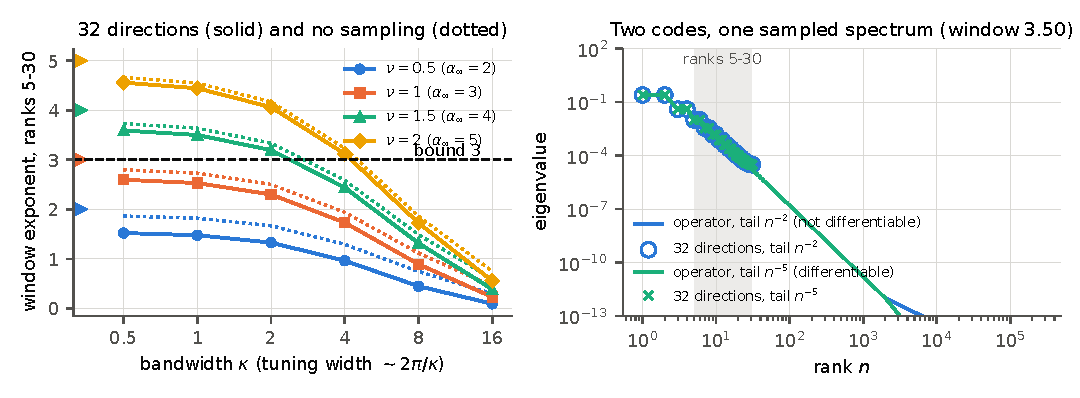
\includegraphics[width=0.94\textwidth]{figures/fig2.pdf}
\caption{Left: ranks 5--30 window exponent for 32 equally spaced directions (solid) and for the operator spectrum without sampling (dotted), against the bandwidth $\kappa$ of the tuning; arrowheads: $\alpha_\infty = 1 + 2\nu$; dashed: the bound 3. Right: the numerical example of Proposition~\ref{prop:window}. Two codes share the differentiable $\nu = 1.5$, $\kappa = 1$ spectrum up to frequency 1,000 and continue as $n^{-2}$ (not differentiable) or $n^{-5}$ (differentiable). Lines: operator spectra; markers: their 32-direction spectra, which coincide; both have window exponent \PropWSmoothA{}, above the bound 3.}\label{fig:d1}
\end{figure}

For every code of the family $c_k = (1 + k^2/\kappa^2)^{-(\nu + 1/2)}$ that we computed, the 32-direction window exponent lies below $\alpha_\infty$, by \GratShortMin{} to \GratShortMax{} (Figure~\ref{fig:d1}). The shortfall has two parts. The operator spectrum is itself shallower than $\alpha_\infty$ over ranks 5--30, by \GratPreMin{} to \GratPreMax{}, because it is flat for frequencies below $\kappa$ and because each frequency carries two equal eigenvalues; even an exact power law $c_k = k^{-3}$ gives \StairThree{} over ranks 5--30. Sampling at 32 directions folds the frequencies above 16 onto lower ones and lowers the exponent by a further \GratAliasMin{} to \GratAliasMax{} (aliasing). The border codes give \GratBorderMin{} to \GratBorderMax{}, all below 3, while differentiable codes with $\nu = 1.5$ give \GratNuOnePointFiveMin{} to \GratNuOnePointFiveMax{} and exceed 3 for $\kappa \le \GratSmoothAboveKappaMax{}$. Within this family and over the bandwidths computed, a 32-direction exponent above 3, such as 3.43, comes only from differentiable codes. Outside the family it does not. In the example of Figure~\ref{fig:d1}, two codes share the $\nu = 1.5$, $\kappa = 1$ spectrum up to frequency 1,000 and continue as $n^{-2}$ (not differentiable) or $n^{-5}$; their tail masses are \PropTailSmoothA{} and \PropTailSmoothB{}, their 32-direction eigenvalues differ by at most \PropRelSmooth{} of the 30th eigenvalue, and both have window exponent \PropWSmoothA{}, the value of the family code: a non-differentiable code gives a 32-direction exponent above the bound. Finite populations of 8,704 neurons changed the 32-direction exponent by at most \GratFinShiftMax{} on average, with a standard deviation of at most \GratFinSDMax{}.

\subsection{The broken-power-law tail exponent}

\begin{figure}[t]
\centering
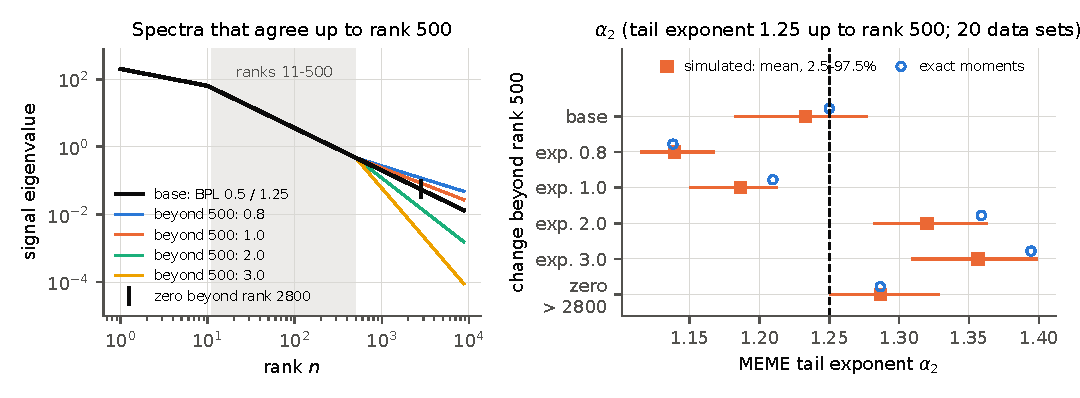
\includegraphics[width=0.94\textwidth]{figures/fig3.pdf}
\caption{Left: the base spectrum, a broken power law with exponents 0.5 and 1.25, and variants that agree with it up to rank 500; shaded: ranks 11--500. Right: MEME $\alpha_2$ (diagonal weights) for each spectrum; squares and bars, mean and 2.5th--97.5th percentiles over 20 simulated data sets with common random numbers; circles, the fit to the exact moments. Dashed: the base tail exponent 1.25.}\label{fig:meme}
\end{figure}

\begin{table}[t]
\centering\footnotesize
\caption{MEME broken-power-law tail exponent $\alpha_2$ for spectra that differ from the base broken power law beyond rank 500 (a different exponent, or zero after rank 2,800) or at every rank (a floor adding 5\% or 15\% of the base variance, or a factor $e^{-n/1000}$). Window: ranks 11--500 exponent of the true spectrum. Trace: variance relative to the base. Exact: fit to the exact moments, diagonal weights (diag.) and full whitening (full). Simulated (diagonal weights): mean $\pm$ standard error over 20 data sets, and the paired difference from the base with its 95\% interval. Flagged: fraction of the 20 data sets whose misfit exceeds the 95th percentile of the correctly specified model, diagonal and full. Last column: the same variants of a base with $\alpha_2 = 1.5$, exact moments, diagonal weights.}\label{tab:meme}
\setlength{\tabcolsep}{2.6pt}
\begin{tabular}{lccccccccc}
\toprule
& & & \multicolumn{6}{c}{base $\alpha_2 = 1.25$} & $\alpha_2 = 1.5$ \\
\cmidrule(lr){4-9}\cmidrule(lr){10-10}
& & & \multicolumn{2}{c}{exact} & \multicolumn{2}{c}{simulated} & \multicolumn{2}{c}{flagged} & exact \\
\cmidrule(lr){4-5}\cmidrule(lr){6-7}\cmidrule(lr){8-9}
change & window & trace & diag. & full & $\alpha_2$ & paired difference & diag. & full & \\
\midrule
none & 1.250 & 1.000 & 1.250 & 1.250 & 1.233 $\pm$ 0.006 &  & 0.05 & 0.00 & 1.500 \\
exponent 0.8 after 500 & 1.250 & 1.142 & 1.138 & 1.144 & 1.139 $\pm$ 0.004 & $-0.094$ [$-0.103$, $-0.085$] & 0.00 & 0.00 & 1.405 \\
exponent 1.0 after 500 & 1.250 & 1.064 & 1.210 & 1.207 & 1.187 $\pm$ 0.004 & $-0.047$ [$-0.054$, $-0.039$] & 0.00 & 0.00 & 1.442 \\
exponent 2.0 after 500 & 1.250 & 0.914 & 1.359 & 1.350 & 1.320 $\pm$ 0.006 & $+0.087$ [$+0.077$, $+0.097$] & 0.00 & 0.00 & 1.529 \\
exponent 3.0 after 500 & 1.250 & 0.879 & 1.394 & 1.386 & 1.357 $\pm$ 0.007 & $+0.123$ [$+0.113$, $+0.134$] & 0.00 & 0.00 & 1.552 \\
zero after 2,800 & 1.250 & 0.950 & 1.286 & 1.289 & 1.287 $\pm$ 0.006 & $+0.053$ [$+0.044$, $+0.063$] & 0.00 & 0.00 & 1.518 \\
\addlinespace
floor 5\% & 1.243 & 1.050 & 1.218 & 1.216 &  & & &  & 1.447 \\
floor 15\% & 1.230 & 1.150 & 1.135 & 1.141 &  & & &  & 1.311 \\
factor $e^{-n/1000}$ & 1.353 & 0.832 & 1.438 & 1.429 &  & & &  & 1.594 \\
\bottomrule

\end{tabular}
\end{table}

The variants in Table~\ref{tab:meme} agree with the base spectrum, a broken power law with tail exponent 1.25, up to rank 500. Beyond it they decay with exponent 0.8, 1.0, 2.0 or 3.0, or stop. Their exact-moment tail exponents range from \MemeTailMinA{} to \MemeTailMaxA{} (from \MemeTailMinB{} to \MemeTailMaxB{} for the base with 1.5): $\alpha_2$ moves toward the true continuation, by at most \MemeTailShiftMax{}, and stays far from it. No window of ranks up to 500 sees these changes. The eigenmoments see them through the trace, which changes by the factor \MemeTraceMin{} to \MemeTraceMax{}; one data set registers this (the log trace has a standard deviation of \MemeSDTrace{}), so the variance in the tail is observed. The moments $p \ge 2$ change by at most \MemeTailZMaxA{} standard deviations. The trace fixes how much variance lies in the tail, not how it decays. With diagonal weights the broken power law absorbs the change into $\alpha_2$: the exact-moment misfits are at most \MemeExactTailMisfitMax{}, against a null median of \MemeNullMedDiag{} and 95th percentile of \MemeNullQDiag{} over \MemeNB{} simulated data sets of the correctly specified model, and no data set of any variant is flagged (of the base, \MemeFlagDiagBaseN{} of 20); the median misfits of the variants, \MemeDiagVarMedMin{} to \MemeDiagVarMedMax{}, are even below that of the base, \MemeDiagBaseMed{}. With full-covariance whitening, closer to the check that Pospisil and Pillow propose (Section~1), the misfit of the correctly specified model has a heavy upper tail: median \MemeNullMedFull{} and 95th percentile \MemeNullQFull{} over the \MemeNB{} base data sets, against \ChiFourMed{} and \ChiFourQ{} for a chi-square distribution with 4 degrees of freedom (eight moments, four fitted parameters counting the profiled break). The five folds have medians \MemeFullFoldMeds{}; the last contributes \MemeFullNullExceedLast{} of the \MemeFullNullExceedAll{} misfits above the pooled 95th percentile, and the largest misfit is \MemeFullNullMax{}. The far-tail variants raise the median misfit of the simulated data sets from \MemeFullBaseMed{} to at most \MemeFullVarMedMax{}. How many of their data sets are flagged depends on the reference: none against the pooled 95th percentile, \MemeFlagFFMin{} to \MemeFlagFFMax{} against the 95th percentile of the first four folds (\MemeFullQFirstFour{}), \MemeFlagFOMin{} to \MemeFlagFOMax{} against that of the first fold, the 20 paired base data sets (\MemeFullQFirst{}), and \MemeLooFlagMin{} to \MemeLooFlagMax{} with the covariance estimated from only 19 data sets (the other paired sets, leaving one out), the exponent-0.8 variant most often. The misfit therefore has little power against these far-tail changes: nominal flag rates run from 0 to \MemeFlagAnyMax{}, depending on the reference distribution and the covariance estimate. The whitened fits shift $\alpha_2$ by similar amounts (exact moments: \MemeFullShiftThree{} for exponent 3.0, \MemeFullShiftPointEight{} for 0.8).

In the simulated data (Figure~\ref{fig:meme}) $\alpha_2$ of the base is \MemeSimBase{} $\pm$ \MemeSimBaseSE{}, with a standard deviation over data sets of \MemeSimBaseSD{}. The far-tail variants shift it by \MemeSimDiffMin{} to \MemeSimDiffMax{} (paired differences). The largest shift, \MemeSimDiffThree{} [\MemeSimDiffThreeLo{}, \MemeSimDiffThreeHi{}] for exponent 3.0, is \MemeRatioThreeSD{} times that standard deviation and \MemeRatioThreeGap{} of the gap of 0.20 between Pospisil and Pillow's average $\alpha_2$ of 1.20 and the natural-image bound of 1; for exponent 0.8 the shift is \MemeSimDiffPointEight{} [\MemeSimDiffPointEightLo{}, \MemeSimDiffPointEightHi{}]. Common random numbers helped only moderately: across data sets the $\alpha_2$ of a variant correlates with that of the base at \MemeCorrMin{} to \MemeCorrMax{}, and the paired differences have standard deviations of \MemePairedSDMin{} to \MemePairedSDMax{} against \MemeSimSDMin{} to \MemeSimSDMax{} for $\alpha_2$ itself. Changes that also touch ranks below 500 can move $\alpha_2$ further: a floor adding 15\% of the base variance lowers the window exponent only to \MemeFloorWinA{} but gives $\alpha_2 = \MemeFloorA{}$ (\MemeFloorB{} around 1.5).

For the Mat\'ern codes of Section~\ref{sec:theory} the relevant input is the set of eigenmoment estimates MEME would compute from their noise-free responses at the 2,800 stimuli (Section~\ref{sec:methods}); these estimate the population moments, not those of the 2,800-stimulus sample spectrum. The weights and the misfit threshold come from the simulated broken power law with neural noise, so for these noise-free moments the misfit is a heuristic filter, not a calibrated test. Many of these spectra are not broken power laws, and the diagonal-weight misfit shows it: its median over the \MemeMaternN{} codes computed is \MemeMaternMisfitMedian{}, far above the null. For $\ell \ge 1$ the profiled break sits at the lower edge of its grid, rank 4, in \MemeBrkLowDiag{} of \MemeBrkLowTotalDiag{} fits with either weighting, and at $\ell = 1/4$ it sits at the upper edge, rank 30, in \MemeBrkHighDiag{} diagonal-weight fits and \MemeBrkHighFull{} full-whitening fit; one diagonal-weight fit ends at the upper limit $\alpha_2 = 6$. These $\alpha_2$ are single-exponent fits from rank 4 onward rather than tail exponents in the usual sense. Among the \MemeGoodN{} fits whose diagonal-weight misfit lies within the null 95th percentile, \MemeGoodSmoothBelow{} of the \MemeGoodSmoothN{} differentiable codes ($\nu = 1.5$) have $\alpha_2$ below the bound and \MemeGoodRoughAbove{} of the \MemeGoodRoughN{} codes with $\nu = 0.75$ have $\alpha_2$ above it, and the border codes fall below it in \MemeGoodBorderBelow{} and above it in \MemeGoodBorderAbove{} cases. The full-whitening misfit passes a different set of \MemeFullGoodN{} fits: \MemeFullGoodSmoothBelow{} of its \MemeFullGoodSmoothN{} differentiable codes lie below the bound, \MemeFullGoodRoughAbove{} of its \MemeFullGoodRoughN{} codes with $\nu = 0.75$ above it, and its border codes \MemeFullGoodBorderBelow{} below and \MemeFullGoodBorderAbove{} above. Under either check, the tail exponents of passing fits lie on both sides of the bound for every smoothness computed. These moments are for infinitely many neurons, while the fit runs over 8,704 indices; for a population of $N$ Gaussian-process neurons $\mathbb{E}\operatorname{tr}\Sigma^2$ exceeds the infinite-population value by a relative amount of about $\mathrm{PR}/N$, with $\mathrm{PR} = (\operatorname{tr}\Sigma)^2/\operatorname{tr}\Sigma^2$ the participation ratio. PR reaches \MemePRMaxQuarter{} at $\ell = 1/4$ in the 8D sets and is at most \MemePRMaxOne{} for $\ell \ge 1$ (a relative change of at most \MemePRRelMaxOne\%). With the moments of a population of 8,704 neurons at $\ell = 1/4$, $\log\operatorname{tr}\Sigma^2$ rises by up to \MemeNLogTwoMax{} (\MemeNLogTwoSD{} weight standard deviations) and $\alpha_2$ changes by at most \MemeNAlphaShiftMax{}; every one of these fits stays below the bound, the number that pass rises from \MemeNPassInfDiag{} to \MemeNPassFinDiag{} of 30 with diagonal weights and from \MemeNPassInfFull{} to \MemeNPassFinFull{} with full whitening, and the statement about both sides of the bound still holds. These fits cover a restricted grid ($\nu \in \{0.75, 1, 1.5\}$, $\ell \in \{1/4, 1, 4\}$).

\subsection{cvPCA bias and the noise level}

The simulations of the preceding analysis found large downward biases of the cvPCA window exponent in conditions whose simulated cvPCA spectra lay far below the calibration recording's in the tail. In the repeated computation (broken power law, $\alpha_2 = 1.5$, realized window slope \SnrTruth{}) the bias was \SnrBiasOne{} $\pm$ \SnrSEOne{} with the calibrated noise, \SnrBiasFour{} $\pm$ \SnrSEFour{} with the non-aligned noise divided by 4, and \SnrBiasSixteen{} $\pm$ \SnrSESixteen{} with it divided by 16. None of the three conditions matches the recording: its cvPCA spectrum at ranks 11, 100 and 500 was (\SnrRatioOne{}), (\SnrRatioFour{}) and (\SnrRatioSixteen{}) times the simulated one in the three conditions, so in every condition the simulated cvPCA spectrum lies below the recording's at these ranks. The bias shrinks in magnitude as the noise is reduced, but we computed no signal-to-noise ratio of the tail, for the simulations or for any recording, so these biases cannot be transferred to the data. It does not bear on identifiability, which concerns the noise-free spectrum.
